%\documentclass[twocolumn]{aastex62}
%\documentclass[manuscript]{aastex62}
%\documentclass[preprint]{aastex62}
%\documentclass[preprint2]{aastex62}
%\documentclass{aastex62}
%\documentclass[twocolumn,tighten,longauthor]{aastex62}
%\documentclass[twocolumn,tighten]{aastex62}
%\documentclass[twocolumn,tighten,longauthor,times]{aastex62}

%\documentclass[a4paper,twoside,10pt]{article}
%\documentclass[preprint,eqsecnum]{aastex62}
%\documentclass[preprint]{aastex62}
\documentclass[a4paper,12pt,modern]{aastex62}

%\usepackage{svn}
%\SVNdate $Date: $
%svn propset svn:keywords 'LastChangedDate' main.tex
\usepackage{fancyhdr}
%\usepackage{datetime}
\usepackage{amsmath}                % American Mathematical Society package
\usepackage{amsfonts}               % American Mathematical Society fonts
\usepackage{amssymb}                % American Mathematical Society symbol
\usepackage{amsthm} 
%\usepackage[pdftex]{graphics}
%\usepackage{graphics,epsf}
\usepackage{graphicx}
\usepackage{epsfig}
\usepackage{epstopdf}
\usepackage{figsize}
\usepackage{natbib}

\usepackage{hyperref}
\usepackage{multirow}
\usepackage[para,online,flushleft]{threeparttable}
\usepackage[super]{nth}
\usepackage[inline]{enumitem}

%\usepackage{draftwatermark}
%\SetWatermarkText{DRAFT}
%\SetWatermarkScale{5}

\renewcommand{\vec}[1]{\mathbf{#1}}
\newcommand{\fracpartial}[2]{\frac{\partial #1}{\partial #2}}
\newcommand{\Lsun}{L_\odot}
\newcommand{\ledd}{L_{\mathrm{Edd}}}
\newcommand{\Rsun}{R_\odot}
\newcommand{\Msun}{M_\odot}
%\newcommand{\lesim}{{<\atop{\sim}}}
\newcommand{\lesim}{\genfrac{}{}{0pt}{2}{<}{\sim}}

\def \kms{~\rm{km~s^{-1}}}
\def \kev{~\rm{keV}}
\def \eV{~\rm{eV}}
\def \cmcub{$\rm{cm}^{-3}$}
\def \msyr{~\rm{M_{\odot}}~\rm{yr^{-1}}}
\def \cm{~\rm{cm}}
\def \s{~\rm{s}}
\def \km{~\rm{km}}
\def \gm{\rm{gm}}
\def \K{~\rm{K}}
\def \g{~\rm{g}}
\def \G{~\rm{G}}
\def \AU{~\rm{AU}}
\def \erg{~\rm{erg}}
\def \yrs{~\rm{yrs}}
\def \yr{~\rm{yr}}
\def \pc{~\rm{pc}}
\def \kpc{~\rm{kpc}}
\def \etc{$\eta$~Car}
\def \days{~\rm{days}}
\def \Jy{~\rm{Jy}}
\def \mum{~\rm{\mu m}}
\def \keV{~\rm{keV}}
\def \astrobj#1{#1}
\def \rmModot{~\rm{M_{\sun}}}
\def \rmRodot{~\rm{R_{\sun}}}
\def \rmLodot{~\rm{L_{\sun}}}
%\def \rmMJ{~\rm{M_J}}
%\def \rmRJ{~\rm{R_J}}

\begin{document}

\title{\LARGE{\textbf{Research Proposal: Simulations of Intermediate Luminosity Optical Transients}}} 
\shorttitle{Research Proposal - Amir Michaelis}
\shortauthors{Research Proposal - Amir Michaelis}


\author[0000-0002-1361-9115]{Amir Michaelis}
\affil{Department of Physics, Ariel University, Ariel, POB 3, 40700, Israel}
\email{amirmi@ariel.ac.il}
\author[0000-0002-7840-0181]{Advisor: Amit Kashi}
\affil{Department of Physics, Ariel University, Ariel, POB 3, 40700, Israel}
\email{kashi@ariel.ac.il}

\date{\today}

%\submitjournal{ApJ}
%\received{XXX}
%\revised{YYY}
%\accepted{ZZZ}



\begin{abstract}

\end{abstract}
%\maketitle

\section{Introduction}
Stars that go transient process are very common phenomena in astrophysics. There is wide range of observation, in particular transient systems that achieves high luminosity. Such a system is for example supernova and nova, thermonuclear eruption, helium shell flashes, born-again models, super Eddington phase objects and many more.
For every object we have the relevant light curve that represent the details of the transient. By taking the total energy of the transient and time of the transient we can draw the Energy-Time Diagram (ETD). Focusing on the Optical Transient Stripe (OTS) in the ETD, that is taking from the light curve the luminosity in the optical and the time duration we can point out a commons objects that form a group which have a common dominate process that is gravitation. This objects that are more luminous than nova but less luminous than supernova (SN) this exotic stellar eruptions known as Intermediate Luminosity Optical Transients (ILOTS). We will discuss the common properties of ILOTs and categories it to types and classes. You can find the different kinds of ILOTs at the ETD figure (see \ref{fig:ilot-club}). You can find up to date ETD figure at \url{phsites.technion.ac.il/soker/ilot-club/} (see figure \ref{fig:ilot-club}). 
\begin{figure}[ht!]
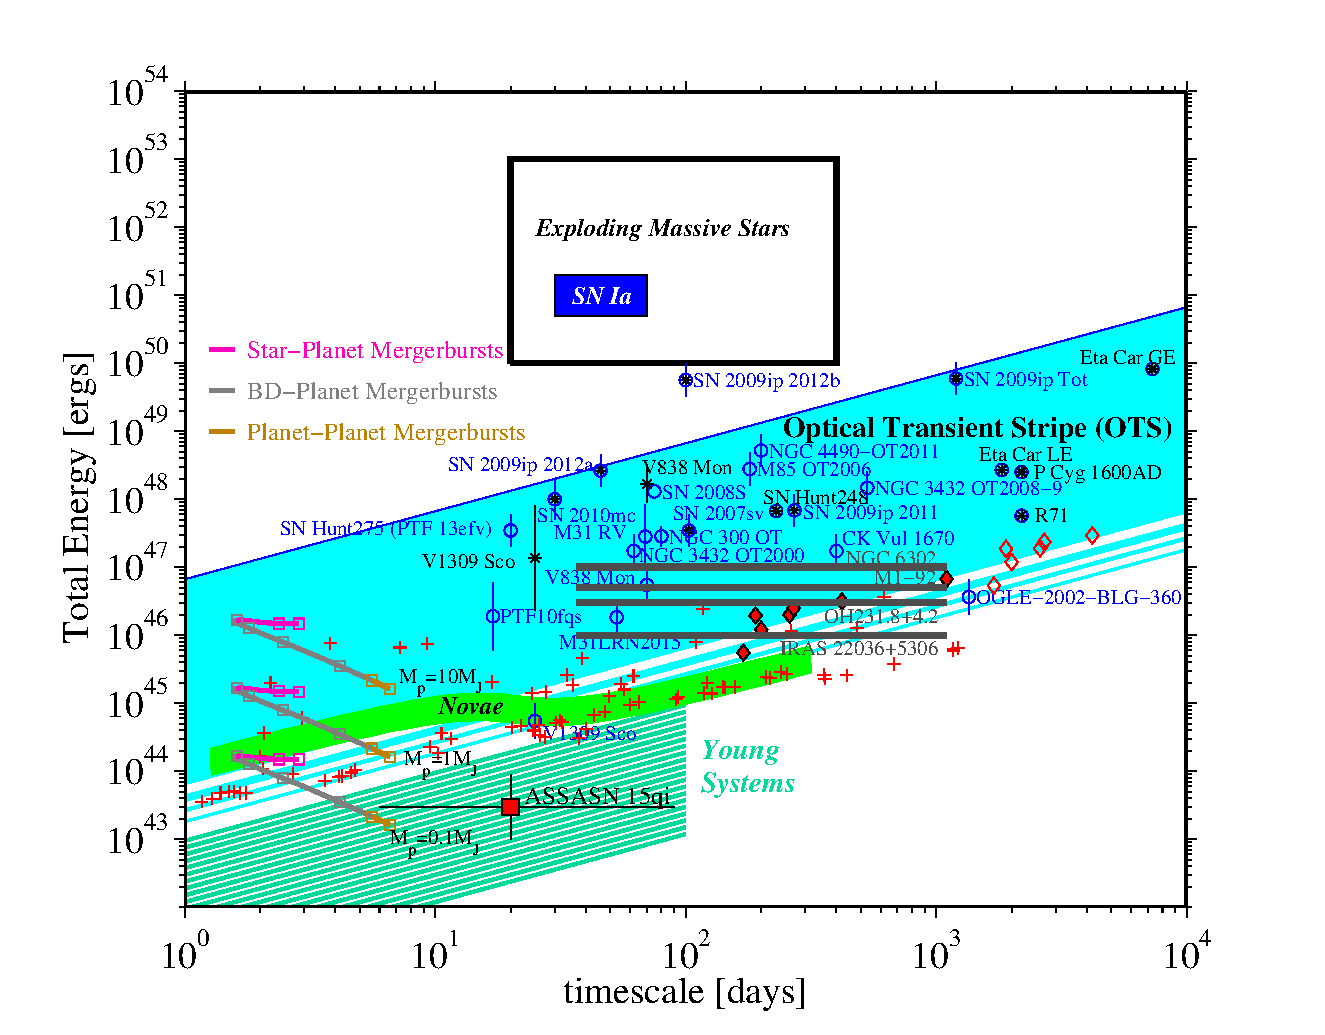
\includegraphics[width=\linewidth]{etd.eps}
\caption{Energy-Time Diagram (ETD) observed transient. The Optical Transient Stripe (OTS), is a more or less constant luminosity region in the ETD. It is populated by Intermediate Luminosity Optical Transients (ILOTs). The observed transient include Width range of processes categorized by types and class, powered by gravitational energy, merger events or vigorous mass transfer events (see \S\ref{subsec:Types of ILOTs}). Blue empty circles represent the total (radiated plus kinetic) energy of the observed transients as a function of the duration of their eruptions. The duration of an eruption is usually (but not always) defined as the time for the luminosity to decrease by 3 magnitudes $\Delta V=-3$. 
Mergerburst events are marked by blue filled circles. Where a model exists to calculate the total available energy, it is marked by a black asterisk above or overlapping the blue circle. The total energy does not include the energy which is deposited in lifting the envelope that does not escape from the star. Where a model exists to calculate the gravitational energy released by the accreted mass (the available energy) it is marked by a black asterisk.
The supernovae region is schematically marked by a rectangle. The green line represents nova models computed using luminosity and duration from \cite{1995ApJ...452..704D}. Nova models from \cite{2005ApJ...623..398Y} are marked with red crosses, and models from \cite{2010ApJ...725..831S} are represented with diamonds.
The four Horizontal lines represent planetary nebulae (PNe) and pre-PNe (Type III ILOTs). The estimated kinetic energies of the components that expand with a linear velocity-distance relation in each of the bipolar planetary nebulae and pre-PNe are marked by horizontal lines. The time scale is an estimate using \cite{2012ApJ...746..100S}.
}\label{fig:ilot-club}
\end{figure}

\subsection{Common Properties of ILOTs}
We plot the light curve at the optical bands for different ILOTs object (types and class) and using a scaling mechanism as describes at \cite{2010ApJ...709L..11K}. The decline from the peak (or peaks) are similar. This behavior strongly implies that the same physical mechanism governs the different objects. We suggest gravitational processes as the govern phenomena. The different objects account for different models (accretion and mergers) witch result in a similar decline. The details of the models and decline rate is of main interest at this proposal. The High Accretion Powered ILOT (HAPI) model shared common properties of many of the ILOTs different models. The model luminosity, as we expected from ILOTs, based on gravitational energy of accreted mass that is partially channeled to radiation. The interaction of the gravitational energy with radiation, emission absorption scattering and re-emission is emitted at the photosphere in the visible light. 

We define $M_a$ and $R_a$ as the mass and radius (respectively) of star `a’ witch accretes the mass and star `b’ as the star that supplies the mass to the accretion. There is various models for different types and classes of ILOTs. For example V838 Mon \cite{2006A&A...451..223T}, NGC300 OT2008-1 \cite{2010ApJ...709L..11K}, $\eta$ Car \cite{2016ApJ...817...66K} and V1309 Sco \cite{2011A&A...528A.114T}.
We can estimate the average total gravitational power as:
\begin{equation} 
L_G=\frac{ G M_a \dot M_a }{R_a}
\end{equation}
The accreted mass creates accretion structure like disk and belt where in a merger star `a’ can dissolve in to the accretion matter. To loss mass due to angular momentum the accretion time should be longer than the viscosity time scale.
The viscosity time scale is scaled according to
\begin{equation} 
T_{visc}\simeq \frac{R^2_a}{\nu} \simeq 73 \left(\frac{\alpha}{0.1}\right)^{-1} \left(\frac{H/R_a}{0.1}\right)^{-1} \left(\frac{C_s/\upsilon_\phi}{0.1}\right) ^{-1} \left(\frac{R_a}{5R_\cdot}\right)^{3/2} \left(\frac{M_a}{8M_\cdot}\right)^{-1/2} \text{days}
\end{equation}
Where $H$ is the thickness of the disk, $C_s$ is the sound speed, $\alpha$ is the disk viscosity parameter, $\nu=\alpha C_s H$ is the viscosity of the disk, and $\upsilon_\phi$ is the Keplerian velocity.  Using $M_a$ and $R_a$ scaled as in \cite{2005A&A...441.1099T} the viscosity to Keplerian timescale become $\chi \equiv t_{visc}/t_k\simeq 160$. We can write the accreted mass as $M_{acc}=\eta_a M_a$. We know from different models that $\eta \lesim 0.1$ with large variation. If we have MS star collides with a star (for example V838 Mon \cite{2006A&A...451..223T}) and tidally disrupts it the destructed star is likely to be less massive than the accretor $M_{acc} < M_b \lesim 0.3M_a$ and $\eta\lesim 0.1$. Another example $\eta\lesim 0.1$ an evolved star loses a huge amount of mass but the accretor gains only a small fraction of the ejected mass (for example the great eruption of $\eta$ Car \cite{2008NewA...13..569K}). 
The viscosity time scale gives an upper limit for the rate of accretion:
\begin{equation}
\dot M_a < \frac{\eta_a M_a}{t_{visc}} \simeq 4\left(\frac{\eta_a}{0.1}\right) \left(\frac{\alpha}{0.1}\right) \left(\frac{H/R_a}{0.1}\right) \left(\frac{C_s/\upsilon_\phi}{0.1}\right) \left(\frac{R_a}{5R_\cdot}\right)^{-3/2} \left(\frac{M_a}{8M_\cdot}\right)^{3/2} \quad M_\cdot yr^{-1}
\end{equation}
The maximum gravitational power is:
\begin{equation}\label{eq.intro.LG}
L_G<L_{max} = \frac{GM_a\dot M_a}{R_a} \simeq 7.7 \times 10^{41}\left(\frac{\eta_a}{0.1}\right) \left(\frac{\chi}{160}\right)^{-1} \left(\frac{R_a}{5 R_\cdot}\right)^{-5/2} \left( \frac{M_a}{8 M_\cdot}\right)^{5/2} \text{erg} s^{-1}
\end{equation}
Where the parameters of the viscosity time scale are replaced with the ratio of the viscosity to the Keplerian time ($\chi$). LHS of equation \ref{eq.intro.LG} represent the top line of the OTS. This luminosity is super-Eddington. For most ILOTs $\eta$ is such that they lay below the supper-Eddington line. Still we see a large variability in $\eta$ and the accretion parameters. Also, we assume thin disk and the picture are much more complicated for thick disk. More accurate treatment requires hydrodynamic simulation together with radiation transfer. This proposal will focus on such solution for a type of problem as describe later in the proposal.

\subsection{Types of ILOTs \label{subsec:Types of ILOTs}}
As we saw earlier the OTS in the ETD is quite wide, containing a range of observation and merger accretion models. They all have in command transient luminosity in the optical govern by gravitational forces. The object ranges from brown dwarf to massive stars. It is only natural we classify them to types and classes \cite{2016RAA....16...99K,2018Galax...6...82K}.

\begin{description}
\item[Type I ILOTs] Type I ILOTs contain three major classes ILRT, LRN and SN impostors (GEs of LBV). These events share many common physical processes mainly they powered by gravitational energy released in a high accretion rate event. The condition for an ILOT to be classified as type I is that the observing direction is such that the ILOT is not obscured from the observer by an optically thick medium.
\begin{description}
\item[Intermediate Luminosity Red Transients (ILRT)] From the Asymptotic Giant Branch (AGB) in particular Red Giant Branch (RGB), the most probable ILOT model where a companion which accretes mass and the gravitational energy of the accreted mass supplies the energy for the eruption. Example include NGC 300 OT \citep{2010ApJ...709L..11K}, SN 2008S and M31LRN 2015.
\item[Giant Eruptions (GEs)] Eruption events of Luminous Blue Variables (LBVs) or other kinds of Very Massive Stars (VMS) mark as atypical SN or SN impostors. GEs ILOTs typically characterize with the highest energy relative to other classes. The energy released in one or sequence of GEs can reach a few $\times10^{46}$ erg. Notice ILRTs are the low mass relatives of LBV GEs. Example include \nth{17} century GE of P~Cyg, \nth{19} century GEs of $\eta$~Car and the pre-explosion eruption of SN 2009ip \cite{2016MNRAS.463.2904S}. 
\item[Luminous Red Nova (LRN) or Red Transients (RT) or Merger Bursts] refers to quite diverse group describing transients powered by complete merger of two stars. During the eruption the observer sees a process of destruction of the less compressed star onto the denser star which is accompanied by the release of gravitational energy that powers the transient this present a characteristic merger light-curve. Example for LRN include V838 Mon \cite{2005A&A...441.1099T} and V1309 Sco \cite{2011A&A...528A.114T} and possible the more massive eruption NGC~4490-OT \cite{2016MNRAS.458..950S}.
\end{description}
\item[Type II ILOTs]  Since most ILOTs are non-spherically symmetric eruptions we can expect that the same transient will seems differently only as a result of the point of view in the sky \cite{2017MNRAS.467.3299K}. This rise a new ILOTs type, binary powered, the Type II ILOTs.
The main classification of this type is obscure point view that is the object line of sight to the observer intersects by a thick dust tours or shell. Such scenario can be strong binary interaction at periastron passage in an eccentric orbit causing strong tidal effects. This trigger the eruption with an unstable outer layer. The interaction leads to an axisymmetrical mass ejection which significantly departs from spherical symmetry. This result with severely attenuates or hides (causing non-direct view) of the binary system or the merger photosphere. This morphology is very common in Planetary Nebulae (PNe) see \cite{1987AJ.....94..671B,1995A&A...293..871C,1996iacm.book.....M,2016JPhCS.728c2008P,2011apn5.confP..21S}. In most cases, the obscuring matter would reside in equatorial directions. The binary system will be obscured to the observer in the optical and IR bands as long as the dust has not dissipated. Type II ILOT is accompanied by some polar mass ejection that may also form dust.
The dust in the polar directions interact with the radiation arrives from the central source. We then can observe this light which becomes much fainter and by doing so making type II ILOTs detectable. A possible example is the outburst observed from the red supergiant N6949-BH1 in 2009 \cite{2017MNRAS.468.4968A}.

\item[Type III ILOTs - Proposed Scenarios for ILOTs] is a collection of classes we expect to exist and populate the empty ETD regions.
\begin{description} 
\item[Weaker Merger burst between a planet and a Brown Dwarf (BD)] This suggested scenario where a planet shredded into a disk around BD and the energy from accretion lead to an outburst \citep{2011MNRAS.416.1965B}. The process is a super-Eddington merger burst occupy the lower part of the OTS on the ETD. In this process the plant destruction occurs before it plunges into the BD. This possible If the average density is smaller than the average density of the BD. The planet must enter the tidal radius of the BD for example a system with highly eccentric orbit gets perturbed. Once the planet is destructed as a result of the sequence of events, the remnant of the merger will resemble other LRNs but on a shorter time scale and smaller energy.

\item[Weak Outburst of a Young Stellar Object (YSO)] YSO undergo unusual outburst like ASASSN-15qi \cite{2016ApJ...831..133H} are similar in many respects to LRN events like V838Mon with lower total energy (much fainter). This ILOTs reside below the OTS. But unlike LRN the secondary object suggested to be Saturn like planet instead of a low mass Main Sequence (MS) companion was tidally destroyed onto the primary YSO \citep{2017MNRAS.468.4938K}. This class include FUor outbursts \cite{2014prpl.conf..387A} witch are pre-MS starts  \cite{1966VA......8..109H,1977ApJ...217..693H} experience an extreme change in magnitude with slow (years) decline and spectral type. FUor more energetic counterparts EXor class of outburst \cite{1989ESOC...33..233H} witch EX Lupis as a prototype \cite{2007AJ....133.2679H}. A pre-MS variables that show flares of a few months to a few years and of several magnitudes of amplitude as a result of episodic mass accretion. Another transient ASASSN-13db \cite{2017A&A...607A.127S} may also be related object.

\item[ILOTs which created a Planetary Nebulae (PNe)]
Noticing similarities between some PNe and ILOTs characteristics \cite{2012ApJ...746..100S} 
\begin{enumerate*}[label={(\alph*)}]
\item a linear velocity-distance relation;
\item a bipolar structure;
\item a total kinetic energy of $\approx 10^{46}-10^{49}$ erg;
\end{enumerate*}
Suggest that this PNe may have formed in an ILOT event lasting a few months where a mass from AGB or ExAGB accrete onto a MS companion. The velocity of the fastest gas parcels in such an outburst will be in the order of the escape speed of the MS star, namely a few $\times100km~s^{-1}$. But most of the gas is expected to interact with the AGB wind and slow down by a factor of 10 (i.e. $\times10km~s^{-1}$). Using simulation \cite{2013MNRAS.436.1961A} in which a very short impulsive mass ejection event from a binary system namely an ILOT developed a PN witch clumpy lobes  quite similar to NGC 6302 demonstrate this process. Example include the PN NGC 6302, the pre-PNe OH231.8+4.2, M1-92, and the IRAS 22036+5306. 
\end{description}
\end{description}

\section{The Model}
To further look into the OS observations, we focus on Type I ILOTs: LRN, RT and merger burst class. We suggest a merger model base on V838 Mon ILOT \cite{2006A&A...451..223T} event.
In this model we have process in which luminosity of $\geq 3\times10^{46}erg~sec^{-1}$ released on a time scale of a month in a pre-main sequence star. 
Unfortunately, there is no well-known process that could achieve such characteristics.
A stellar merger scenario that can result in the require light-curve is suggested and model that can simulate the process is propose.
Gravitation, in particular accretion, events especially into compact object are very efficient in terms of energy liberated per unit mass accreted.
Accretion on main sequence star with luminosity of $\sim 10^6 ~ L_{\odot}$ result with accretion rate of $\geq 0.01M_{\odot}yr^{-1}$.
Applying this to V838~Mon we need to accrete $\geq 0.1 M_\cdot$ on a time scale of months.
During the main outburst of V838~Mon (January - mid April 2002) the system lost $\sim2.5\times10^{46}$ergs in radiation and presumably $0.01-0.1 M_\odot$ in mass loss (observe by lines) with velocities of $300km~sec^-1$.
The energy necessary to lift this matter from the surface of a star having $M_{\star}=8M_\odot$ with $R_{\star}=5R_\odot$ and to accelerate it to $300km~sec^{-1}$ at large distances is $(0.4-4)\times 10^{47}$ ergs.
Binary system can't generate the desire light curve as there no mechanism to accrete on very short time such amount of mass.
The only process that can came close is young main sequence stellar or pre main sequence stellar surrounded with massive protostellar disc.
Thermal instabilities in the disc, similar to those in dwarf novae, can transfer a significant mass from the disc to the central star.
This mechanism believed to produce FU~Ori type eruptions \cite{1996ARA&A..34..207H}.
The Disc in FU~Ori type objects can transfer as much as $0.01M_\odot$ on time scale of hundred years.
For the V838~Mon event (time scale of mounts) and assuming the system is young that there is in addition to the binary start, main sequence and much smaller companion (we see in the decline phase as B3V star), with a protostellar disc that interact with the smaller star resulting with high eccentric orbit, see for example \cite{1991ApJ...370L..35A} for stellar binaries or in \cite{2002MNRAS.330L..11A} for migrating brown dwarfs around low mass stars, leading to a merger with the primary.

\subsection{Propose Simulation}
we will use version 4.5 of the \textsc{flash} hydrodynamic code \cite{2000ApJS..131..273F}. It is a well-tested publicly available multiphysics multiscale simulation code with a wide international user base routinely used by many astrophysicists. It has a wealth of documentation, help resources and complementary tools. It is an Eulerian hydrodynamics code with adaptive mesh refinement (AMR) including robust solvers for hydrodynamic like the well-known piecewise-parabolic method (PPM) \cite{1984JCoPh..54..174C}. Alongside \textsc{flash} we will use RADMC-3D\footnote{\url{http://www.ita.uni-heidelberg.de/ dullemond/software/radmc-3d/}} \cite{2012ascl.soft02015D} a freely available and open source Monte Carlo radiative transfer code a used in astronomy and astrophysics. It calculates, for a given geometrical distribution of gas and dust, what its spectra look like when viewed from a certain angle. The code is well documented and has numerous simple examples that can be used as templates. Orchestrate the two, and for visualization we will use the yt-project \cite{2011ApJS..192....9T} integrated science environment for collaboratively asking and answering astrophysical questions. To do so, it will encompass the creation of initial conditions, the execution of simulations, and the detailed exploration and visualization of the resultant data. It will also provide a standard framework based on physical quantities interoperability between codes. Yt is driven by a commitment to Open Science principles which include a friendly and helpful community of users and developers, and Free and Libre Open Source Software.

Our goal is to simulate a primary star with protostellar disk and much smaller companion.

\subsection{Setup}
\label{sec:setup}
We setup initial conditions of star that had just underwent a merger burst.
The star disk originated from the destruction of the companion is a thick disk.
The disk mass will be $0.1-1 M_\odot$ it will be covering a semi-angle of $30 \deg$ around the equator with radius of about  $R\sim10-15 AU$ forming a torus.
The primary star mass is $8 M_\odot$ and its radius is $5 R_\odot$.
We use for the initial condition a gas dominate spinning tours in a Keplerian velocity follow the thick disk model \cite{ 2002apa..book.....F} Ch.10 and Ch.11 (see \S\ref{app:thick_disk_model}).

The initial disk temperature is about $10^4~K$ similar to the companion photosphere temperature. The disk composition also taken from the companion star to be $X\sim0.7$ and $Y\sim0.28$.
The following initial disk dimensionless parameters holds and give better understanding of the fluid flow: 
\begin{enumerate*}[label={(\alph*)}]
\item Toomre’s parameter \cite{1964ApJ...139.1217T} $Q=\frac{c_s\kappa}{\pi G \Sigma} > 1$, the disk is gravitationally stable.
\item Reynolds numbers $R_e=\rho u l / \mu>>1$.
\item Knudsen number $K_n=\lambda_\gamma / R$, where $\lambda_\gamma$ is the gas mean free path.  We can use continuum mechanics to describe the problem.
\item Magnetic Reynolds number $R_{en}= c_s H/ \eta <<1$, where $\eta$ is the magnetic diffusivity of the fluid.  We can assume the Magneto-Hydro-Dynamic (MHD) effects are small.
\end{enumerate*}

We expect the disk to undergo instabilities \citep{1988MNRAS.232....1F},("Accretion Flows in Astrophysics"; 2018;Nikolay Shakura) such that part of the gas in the disk will be dissipated and part of the gas in the disk will be accreted onto the primary star.
We will be able to quantify the accretion rate and identify the directions from where the accreted material arrives onto the star similar to \cite{2018arXiv180502529K,2018Galax...6...82K}.

Using \textsc{flash} simulation we will take frequent snapshot and postprocess them in RADMC-3D.
This will able us to derive Spectral Energy Distribution (SED), and determine the luminosity as a function of time in each waveband (in optical and near-IR) as seen by an observer.
We will test different lines of sight, as the same eruption can look very different from different lines of sight \cite{2017MNRAS.467.3299K}.
This will allow us to compare the simulate transient light curve to the observed one.
We will test many parameters to cover as much as possible of the parameters space. E.g, different masses in the disk, covering fraction of the disk (angle), artificial viscosity values etc.

\section{Road-Map}

In order to reach our goals, we presents the project main checkpoints.
\begin{enumerate}
\item Linux developer machine running \textsc{flash}, RADMC-3D, Visit, yt-project and all the companion software development environments like openMPI, HDF5, IDEs and much more.
\item Run \textsc{flash} hydrodynamic 3D test code on coarse grid. Run the tori Keplerian rotating test case. Use Visit to inspect the result.
\item Add more physics to the test case like multi-species, multi-gamma equation of state and radiation transfer.
\item Integrate RADMC-3D code \citep{2012ascl.soft02015D} for post-processing.
\item Add yt visualization support.
\item Manage the simulation using python. Run \textsc{flash} and RADMC-3D automatically from python. Run some hydrodynamic steps then do RADMC-3D post-processing and continue with the simulation alternately to get a wide observation like picture.
\item Debug and test the code (reliability) on coarse grid.
\item Port the code to a high power computer (HPC), based on open MPI. Running the thick disk accretion model on a fine grid.
\item Full scale running.
\item Analyze the results and summarize the result.
\item Explore the model relevant parameter space.
\end{enumerate}

%\section{Methods}

\appendix
\section{Preliminary result\label{app:preliminarty result}}
We present the initial result of the simulation discussed in section \S\ref{sec:setup}. This appendix shows we have the require expertise to setup and run the require simulation. It shows only the first step into the simulation at low resolution has we leak the HPC resource at this time. We present a \textsc{flash} setup with central star of $8M_\odot$ in the center surround with thick accretion disk, a torus like, of $1M\odot$ with Keplerian velocities. In figure \ref{fig:preliminary-result-density} we can see the border lines of the density as a iso-surface color with red and the Keplerian velocity between the upper and lower surface showing the disk matter movement. The green circular glyphs represent the Keplerian velocity of the thick disk. The density distribution in the disk is small and we discard their iso-surface for clarity. In the upper view we see a blue glyphs represent the ISM, a very low density region about $\sim10^{-10} gm/cm^3$, attract to the central object. The ISM start with no velocity and quickly fall into the central object. Figure \ref{fig:preliminary-result-velocity} show the same snapshot of the simulation focus on the velocity field.  

\begin{figure}[ht!]
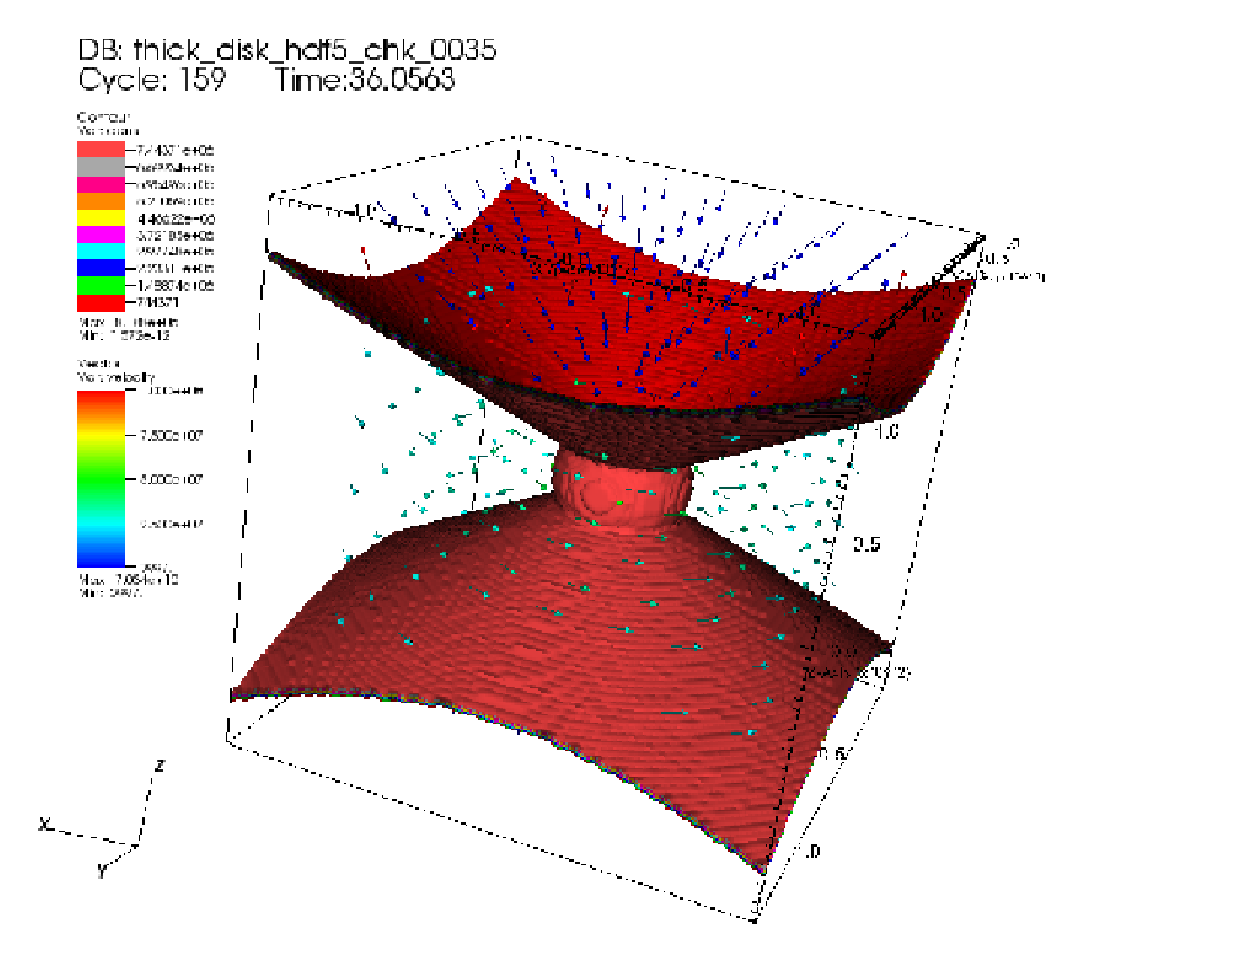
\includegraphics[width=\linewidth]{visit_dens_1.eps}
\caption{The simulation snapshot after a few steps showing the system setup. The iso-surface of the density color with red. The volume between the surfaces are filled with matter and the variation in the density is very small so we discard the relevant iso-surfaces for clarity. The matter between the surfaces form the thick disk and it initially set to Keplerian velocity distribution. The matter outside the surfaces are filled with ISM like matter with no velocity.}\label{fig:preliminary-result-density}
\end{figure}

\begin{figure}[ht!]
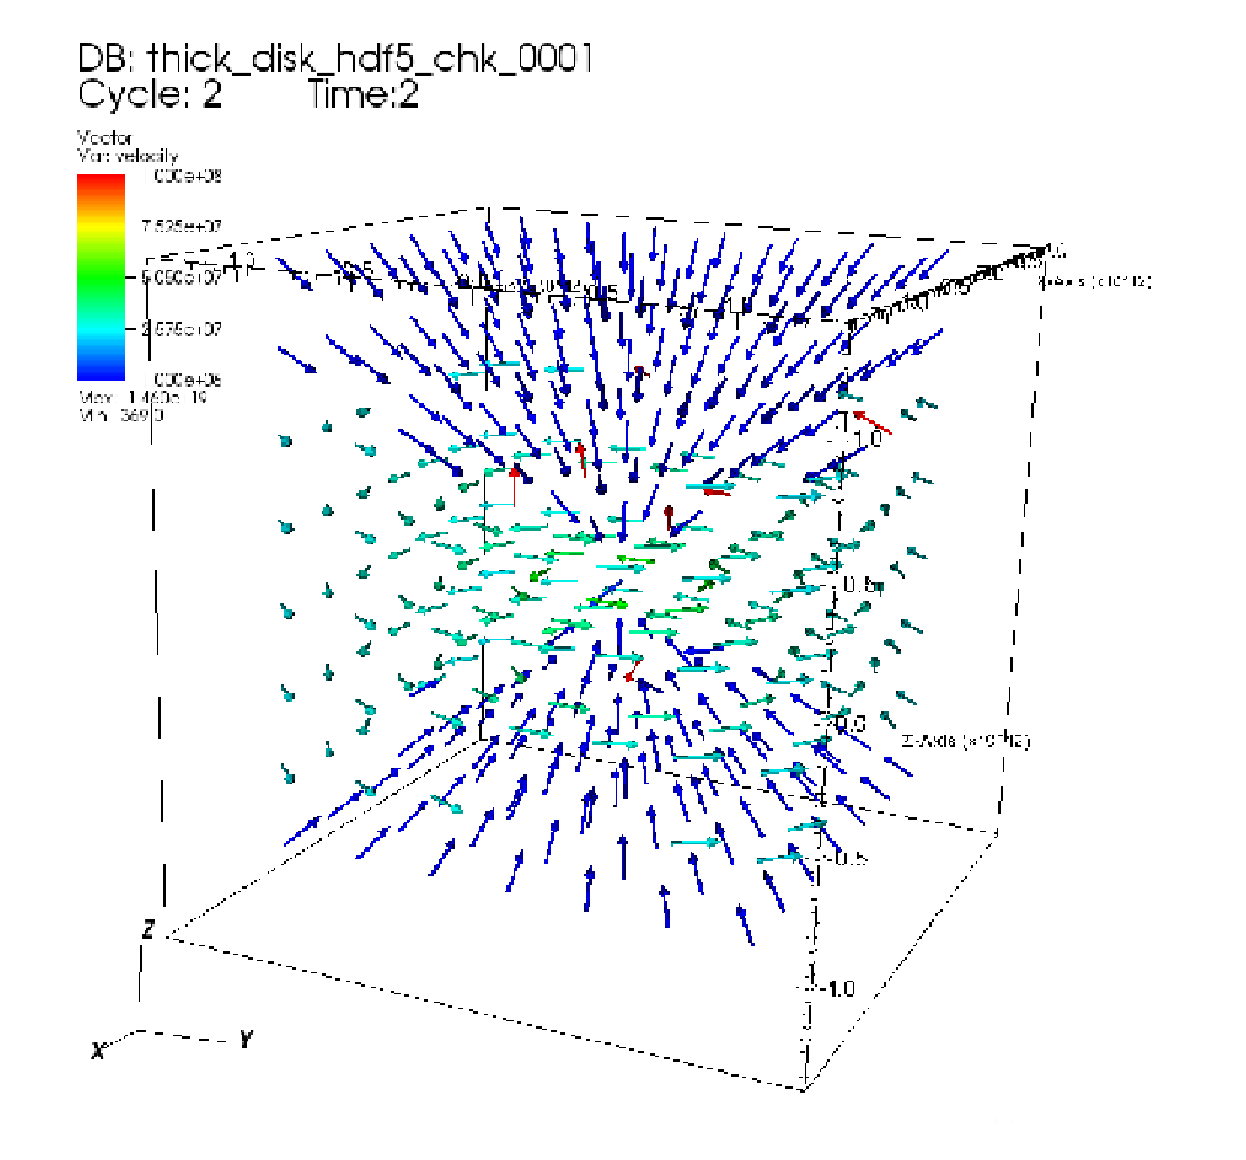
\includegraphics[width=\linewidth]{visit_vel_1.eps}
\caption{In this figure we focus on the velocity field. The green glyphs are the thick disk Keplerian distribution and the blue glyphs represent the ISM matter fall into the central object as it start with zero velocity.}\label{fig:preliminary-result-velocity}
\end{figure}


%\section{Polytropic Envelope\label{app:polytropic_envelope}}
%TBA

\section{Thick Disk Model\label{app:thick_disk_model}}
In this appendix we present the thick disk model as discussed in literature. The case of thick disk is still under development and rises theoretical and observational questions. There is a large number of works indicating that thick disk plays an important role in AGN. There also indication that thick disk rise in stellar merger, generation of bipolar outflows and jets and early stages of star formation.
As a result there isn't a well-known agreed upon `textbook' thick disk solution, instead there is a well-known guideline of the tori model.
We follow \cite{2002apa..book.....F} book, but first let us present a few hydrodynamic governing equations.

We start with conservation of mass (continuity equation),
\begin{equation}\label{eq:conservation_of_mass}
\frac{\partial \rho}{\partial t} + \frac{\partial (\rho u_k)}{\partial x_k} = 0
\end{equation}
Where $\rho$ is the matter density and $u_k$ is the fluid velocity.

We continue on to conservation of momentum,
\begin{equation}\label{eq:conservation_of_momentum}
\rho\frac{\partial u_j}{\partial t} + \rho u_k \frac{\partial u_j}{\partial x_k}=\frac{\partial \sigma_{ij}}{\partial x_i}+\rho f_j
\end{equation}
Where $f_i$ is body forces per mass, $\sigma_{ij}$ defined as, 
\begin{equation}
\sigma_{ij} \equiv -p\delta_{ij}+\tau_{ij}
\end{equation}
p is the pressure and $\tau$ is the shear stress tensor
\begin{equation}
     \tau_{ij} = \lambda \delta_{ij} \frac{\partial u_k}{\partial x_k}+ \mu \left( \frac{\partial u_i}{\partial x_j} + \frac{\partial u_j}{\partial x_i} \right)
\end{equation}
$\lambda$ and $\mu$ are the dynamic viscosity and second viscosity coefficient. Usually the kinematic viscosity defined as $\nu = \mu/\rho$. The second viscosity coefficient can be represent as $\lambda = \K - 2\mu/3$, $\K$ is the bulk viscosity defined as
\begin{equation}
    p-\bar p = \K \frac{\partial u_k}{\partial x_k} 
\end{equation}
which for incompressible fluid lead to stokes relation $\lambda = - 2\mu/3$.

The conservation of energy is,
\begin{equation} \label{eq:conservation_of_energy}
\rho\frac{\partial e}{\partial t}+\rho u_k \frac{\partial e}{\partial x_k} = \sigma_{ij} \frac{\partial u_j}{\partial x_i} - \frac{\partial q_j}{\partial x_j}
\end{equation}
Where $e$ is the intrinsic energy of the fluid per mass and 
\begin{equation}
q_j \equiv -\kappa \frac {\partial T}{\partial x_j}    
\end{equation}
is the heat flux leaving the fluid, $\kappa$ is the thermal conductivity of temperature.

The set of equations \ref{eq:conservation_of_mass}, \ref{eq:conservation_of_momentum} and \ref{eq:conservation_of_energy} with two equation of state $p=p(\rho,T)$ and $e=e(\rho,T)$ named the Navier-Stokes equations. 
The disk equation (and \textsc{flash}) derived from this set of equations with different physics lead to different terms and approximations (different representation of the equation).
For more detailed discussion on fluid flow see \cite{currie2002fundamental}.

%Equipped with Navier-Stokes we move to toroidal equilibria without accretion solution (\cite{2002apa..book.....F} Ch.10) as a representation of thick disk.
Thick disk might form during the merger of two stars as the system attempts to handle its excess angular momentum.
As we shall see, these thick disk may possess a narrow funnel along the rotation axis where large radiative pressure gradients can accelerate matter in collimated jets. 
Thus the appeal of thick disk resides in the feasibility of a model which derives its power from accretion and intrinsically generates jets without any extra assumptions (e.g. magnetic fields, a confining cloud, etc).

We start by describing the structure and shape of pure (with no viscosity) rotating fluid in about its axis of symmetry in cylindrical system of coordinates $(R,\phi,z)$. 
Then the velocity field has the components: 
\begin{equation}\label{eq:velocity_field_components}
V_R=0, \quad v_\phi=R\Omega, \quad v_z=0
\end{equation}
Where $\Omega$ is the angular velocity (i.g. for thick Keplerian disk $\Omega=\sqrt{G M_\star / R^3}$).
Navier-Stokes equations for inviscid fluid in cylindrical coordinates reduce to
\begin{equation}
% equations of motion of an inviscid fluid subject to gravitational forces (including external bodies)
\begin{split}
\label{eq:inviscid_fluid}
\frac{1}{\rho} \frac{\partial P}{\partial R} = - \frac{\partial \Phi}{\partial R} + \Omega^2R,  \\
\frac{1}{\rho} \frac{\partial P}{\partial R} = - \frac{\partial \Phi}{\partial z}
\end{split}
\end{equation}
Where $P$ is the pressure and $\Phi$ is the gravitational potential.
Notice that the equations in vector form are:
\begin{equation}\label{eq:vector_inviscid_fluid}
\frac{1}{\rho}\mathbf{\nabla} P = -\mathbf{\nabla}\Phi+\Omega^2\mathbf{R} = \vec{g_{eff}}
\end{equation}
We defined the effective gravity $\vec{g_{eff}}$ as the vectorial sum of gravitational and centrifugal acceleration. Therefore the isobaric surface is perpendicular to $\vec{g_{eff}}$ at any point.
So we can write along the isobaric surface (denote by subscript s):
\begin{equation}
\frac{\partial g_{eff}}{\partial R} dR_s + \frac{\partial g_{eff}}{\partial z} dz_s =0
\end{equation}
Using \ref{eq:inviscid_fluid} along the definition of effective gravity we get:
\begin{equation}\label{eq:surface_differential}
\left( \Omega^2R \right)_s = \left( \frac{\partial \Phi}{\partial z} \right)_s \frac{\partial z_s}{\partial R_s} + \left( \frac{\partial \Phi}{\partial R} \right)_s
\end{equation}
Now suppose a cloud of negligible mass rotates around a point mass $M_\star$ with angular velocity $\Omega$ such that 
\begin{equation}
\Omega^2=\frac{GM_\star e^2}{r^3}=\frac{GM_\star e^2}{(R^2+z^2)^{3/2}}
\end{equation}
With $\Phi=-GM_\star/r$ we can integrate directly equation \ref{eq:surface_differential} to yield the meridional cross-section of our disk
\begin{equation}
(1-e^2)R^2+z^2=constant=z^2_P
\end{equation}
This result indicate $P=P(z_P)$ and from equation \ref{eq:inviscid_fluid} we can solve for the density:
\begin{equation}
\frac{1}{\rho}=-\frac{\partial \Phi}{\partial z} / \frac{\partial P}{\partial z}
\end{equation}
Which lead to 
\begin{equation}
\frac{\partial P}{\partial z} = \frac{\partial P}{\partial z_P}\frac{\partial z_P}{\partial z} = \frac{\partial P}{\partial z_P}\frac{z }{z_P}
\end{equation}
Thus obtain for the for the density
\begin{equation}
\frac{1}{\rho}=-\frac{GM_\star z_P}{r^3(dP/dz_P)}
\end{equation}
From this result we see that physically plausible equilibria require $dP/dz_P<0$ (i.e. pressure must decrease outwards to balance gravity). 
Activate the curl operator ($\mathbf{\nabla}\times$) on equation \ref{eq:vector_inviscid_fluid} and using  \ref{eq:velocity_field_components} we yeild
\begin{equation}
    \vec\nabla\left(\frac{1}{\rho}\right)\times\vec\nabla P = 2\Omega \vec\nabla \Omega \times \vec R = 2\frac{\partial \Omega}{\partial z} \vec v
\end{equation}

 The vectors $ \vec\nabla\left(\frac{1}{\rho}\right)$ and $\vec\nabla P$ are orthogonal to isopycnic (constant density surface) and isobaric surfaces respectively. If $\partial \Omega/ \partial z=0$ everywhere result with the two vectors must be parallel everywhere, the surfaces of constant pressure and constant density are coinciding and this also implies that $\Omega=\Omega(R)$ for non-vanishing rotation. This result simplifies considerably the task of finding the structure of the disk when the angular velocity is constant on cylinders. Also anther immediate result is that the pressure and density must be functionally related $P=P(\rho)$.
As result of $\partial \Omega/ \partial z=0$ it is possible to introduce a rotational potential $\psi_{rot}$ such that
\begin{equation}
\Omega^2(R)\vec R = \vec \nabla \psi_{rot}
\end{equation}
Where 
\begin{equation}
\psi_{rot} = \int^R  \Omega^2(R') R' d R'
\end{equation}
Then form equation \ref{eq:vector_inviscid_fluid} we have $\Phi_{eff}=\Phi-\psi_{rot}$ and $\vec g_{eff} = -\vec \nabla \psi_{eff}$ so that the equation for isobaric/isopycnic surface becomes simply 
\begin{equation}\label{eq:phi_eff_constant}
\Phi_{eff}=constant
\end{equation}
In this configuration the surfaces of constant pressure, density and effective potential all coincide. Therefore finding the shape and stratification of the disk is reduced to obtaining the equipotentials of $\Phi_{eff}$. As we know a priori the gravitational potential this task is relatively simple. So we may use $\Phi_{eff}=\Phi(R,z)-\psi_{rot}(R)=constant$ to obtain the equlibrium rotation field for a given equipotential shape resutl with:
\begin{equation}\label{eq:rotation_potantial}
    \psi_{rot}=\Phi(R,z_s(R))
\end{equation}
where $z=z_s(R)$ is the equation for the cross-section of the surface. Now consider a disk surface generated by revolution of two straight lines at angles $\pm\alpha$ to the equatotial plane. Let us assume the disk self gravity is negligible and it is in equilibrium with the gravitational field of point mass $M_\star$ at the origin.
The equation for the cross-section of the disk angular half-thickness $\alpha$ is
\begin{equation}
z_s(R)=\pm(\tan\alpha)R
\end{equation}
As all the conditions required for the validity of \ref{eq:rotation_potantial} are met, we subsitute this into the potential of the point mass to obtain
\begin{equation}
    \psi_{rot}(R)=GM_\star\cos\alpha/R
\end{equation}
and for angular velocity 
\begin{equation}\label{eq:angular_velocity}
    \omega^2=\frac{1}{R}\frac{\partial \psi_{rot}}{\partial R} = \frac{GM_\star\cos\alpha}{R^3}
\end{equation}
The equilibrium rotation field is `Keplerian' but corresponds to a mass $M_\star\cos\alpha<M_\star$, where the velocities are less then Keplerian velocities because the pressure distribution necessary to support the disk vertically has a radial gradient. From \ref{eq:phi_eff_constant} where we set $\Phi_{eff}\neq0$ we get one parameter family $\Phi_{eff}$ for the internal pressure and density stratification layers
\begin{equation}
    r=\left[ GM_\star/(-\Phi_{eff})\right] \left(1-\cos\alpha/\cos\lambda \right)
\end{equation}
where $\lambda$ is the latitude. 
For small values of $\alpha$ we notice that $|\partial P/\partial z| \gg |\partial P/\partial R|$ this result also characterize a range of thin accretion disk.
\begin{figure}[ht!]
\includegraphics[width=\linewidth]{meridional_equipotentials_section_z–R_plane_thick_disk.png}
\caption{Meridional equipotentials section in the z–R plane, surface given
by $z_s=\pm(\tan \alpha)R$. The bound fluid $E < 0$ is shown shaded.}
\label{fig:thick-disk-tori-struct}
\end{figure}

After gaining some insight into the thick disk geometrical structure, we pursue some details about the disk luminosity. We show that disk can grow beyond (exceed) Eddington limit by large factors. If the disk contains a hollow axial region (this is true for a large class of thick disk objects), commonly known as the `funnel’, in this region the centrifugal force always exceeds gravity such that the balance between the pressure gradients and rotation determines the disk equilibrium.
As it turns out the maximum radiative output in this thick disk funnels objects related to rotation rather than to the central mass and therefore can exceed $L_{Edd}$.
Before we begin let us make some order of magnitude estimation. 
For nuclear processes ($H\rightarrow He$) we can get about $\sim 0.007~mc^2$ in energy, for accretion we can have $\sim R_{sch}/(2R) ~mc^2$ where for example $R<70R_{sch}$ we get $\sim 1/(2\cdot 70) ~mc^2 \sim 0.05~mc^2$. That is accretion process can easily be more efficient. 
The radiation force can roughly be estimate as 
\begin{equation}
F_{out}=\frac{\sigma_T L_\star}{4\pi r^2 c}
\end{equation}
Where we use Thomson scattering (ionized hydrogen of free electrons) cross section $\sigma_T=6.7\dot10^{-25} ~cm^2$.
The inward balancing gravitational force on the electron proton pair is 
\begin{equation}
F_{in}=\frac{GM_\star m_p}{r^2}
\end{equation}
Comparing the two result with Eddington luminosity 
\begin{equation}
L_{Edd} = \frac{4\pi G M_\star m_p c}{\sigma_T}\approx 3.4\cdot 10^4 L_\odot \left( \frac{M_\star}{M_\odot} \right)
\end{equation}
If the entire gravitational energy emitted as radiation 
\begin{equation}
L_{acc} = \frac{G M_\star \dot M}{R_\star}
\end{equation}
And taking in to account the Eddington limit we get
%\begin{equation}
%\begin{split}
%\dot M_{Edd} = \frac{4\pi m_p c R_\star}{\sigma_T} \\
% %\dot M_{Edd} \approx 9\cdot10^{16} gram~sec^{-1} %\left(\frac{R_\star}{1 ~km}\right) \\
%\dot M_{Edd} \approx 1\cdot10^{-1} M_\odot ~Yr^{-1} \left( %\frac{R_\star}{R_\odot} \right)
%\end{split}
%\end{equation}
\begin{equation}
\dot M_{Edd} = \frac{4\pi m_p c R_\star}{\sigma_T}
\end{equation}

\begin{equation}
\dot M_{Edd} \approx 1\cdot10^{-1} M_\odot ~Yr^{-1} \left( \frac{R_\star}{R_\odot} \right)
\end{equation}
We can define the disk black-body temperature as
\begin{equation}
T_b=(L_{acc}/4\pi R_\star^2 \sigma)^{1/4}
\end{equation}
and the disk thermal temperature as ($3kT\simeq GM_\star m_p / k R_\star$)
\begin{equation}
T_{th}=GM_\star m_p /3 k R_\star
\end{equation}
in general we have
\begin{equation}
T_b \leq T_{rad} \leq T_{th}
\end{equation}
for optically thick disk radiation is in equilibrium with the thermal temperature $T_{rad}\sim T_{th} \sim T_b$ .

The radiative flux in equilibrium can be write as
\begin{equation}
\mathbf{F}= -\frac{C}{\kappa \rho}\mathbf{\nabla}P_{rad}
\end{equation}
Where $\kappa$ is the opacity per unit mass. The maximum radiation attain when the effective gravitation is balanced by the radiation, and using \ref{eq:vector_inviscid_fluid} we obtain
\begin{equation}\label{eq:Fmax-rad}
    \vec F_{max} = -\frac{c}{\kappa}\vec g_{eff} = \frac{c}{\kappa}\vec\nabla\Phi - \frac{c}{\kappa}\vec \Omega^2(R,z)\vec R
\end{equation}
The maximum luminosity achieve by simply inegrated $F_{max}$ over the entire surface of the body.
\begin{equation}
    L_{max} = \frac{c}{\kappa} \int_S \vec\nabla\Phi\cdot d\vec S + \frac{c}{\kappa}\int_S \Omega^2\vec R \cdot d\vec S
\end{equation}
or using Gauss theorem 
\begin{equation}
    L_{max} = \frac{c}{\kappa} \int_V \nabla^2\Phi dV + \frac{c}{\kappa}\int_V \vec\nabla(\Omega^2\vec R) dV
\end{equation}
Remembering Poisson's equation $\nabla^2\Phi=4\pi G \rho$ where $\rho$ is the matter density of the sources of $\Phi$. We focus on the second term and using \ref{eq:velocity_field_components}
\begin{equation}
    \vec\nabla(\Omega^2\vec R) = \vec R \cdot \vec\nabla\Omega^2 + \Omega^2(\vec\nabla\cdot\vec R) = 2R\Omega \frac{\partial\Omega}{\partial R} + 2\Omega^2
\end{equation}
Writing the last equation using the completing squares,
\begin{equation}
    \vec\nabla(\Omega^2\vec R) = \frac{1}{2}\left[ \frac{1}{R}\frac{\partial}{\partial R}(R^2\Omega) \right]^2 - \frac{1}{2} \left( R\frac{\partial \Omega}{\partial R} \right)^2
\end{equation}
Where the first term represent the square of the z-component of the vorticity $\omega = \mathbf{\nabla} \times \mathbf{v}$, and the second term related to the shear.
Thus, collecting result
\begin{equation}
    L_{max}=\frac{4\pi G M c}{\kappa}+
    \frac{c}{2\kappa}\int_V \left( R\frac{\partial \Omega}{\partial R} \right)^2 dV -
    \frac{c}{2\kappa}\int_V \left[ \frac{1}{R}\frac{\partial}{\partial R}(R^2\Omega) \right]^2 dV
\end{equation}
Where $M$ is the mass of the disk and not the central object.
The first term is the well-known Eddington limit.
The second term relate indirectly to the central object by rotation and contain the shear which makes the dominant contribution enabling $L_{max}$ exceed $L_{Edd}$. The third term containing the vorticity always reduces $L_{max}$ unless the angular momentum per unit mass $l=RV_\phi=R^2\Omega$ is independent of $R$.
We now will work out the maximum luminosity that can be emitted between two radii $R_1$ and $R_2$. We can achieve this by direct integration of $F_{max}$ over both sides of the disk.
\begin{equation}
    L_{max}=2\int_{R_1}^{R_2} F_{max} (2\pi R/cos\alpha) dR
\end{equation}
We can evaluate the integral using \ref{eq:angular_velocity} and \ref{eq:Fmax-rad} or directly by using simple geometry see figure \ref{fig:simple_geometry_geff_Lmax}.
\begin{equation}
    F_{max}=\frac{c}{\kappa} g_{eff} = \frac{c}{\kappa}g\tan\alpha
\end{equation}
Where $g=GM/r^2$ is the gravitational acceleration and $R=r\cos\alpha$.
Result with,
\begin{equation} \label{eq:L_max_exceed_L_eddingtion_R1R2}
    L_{max}=L{Edd}\sin\alpha \ln (R_2/R_1)
\end{equation}
\begin{figure}[ht!]
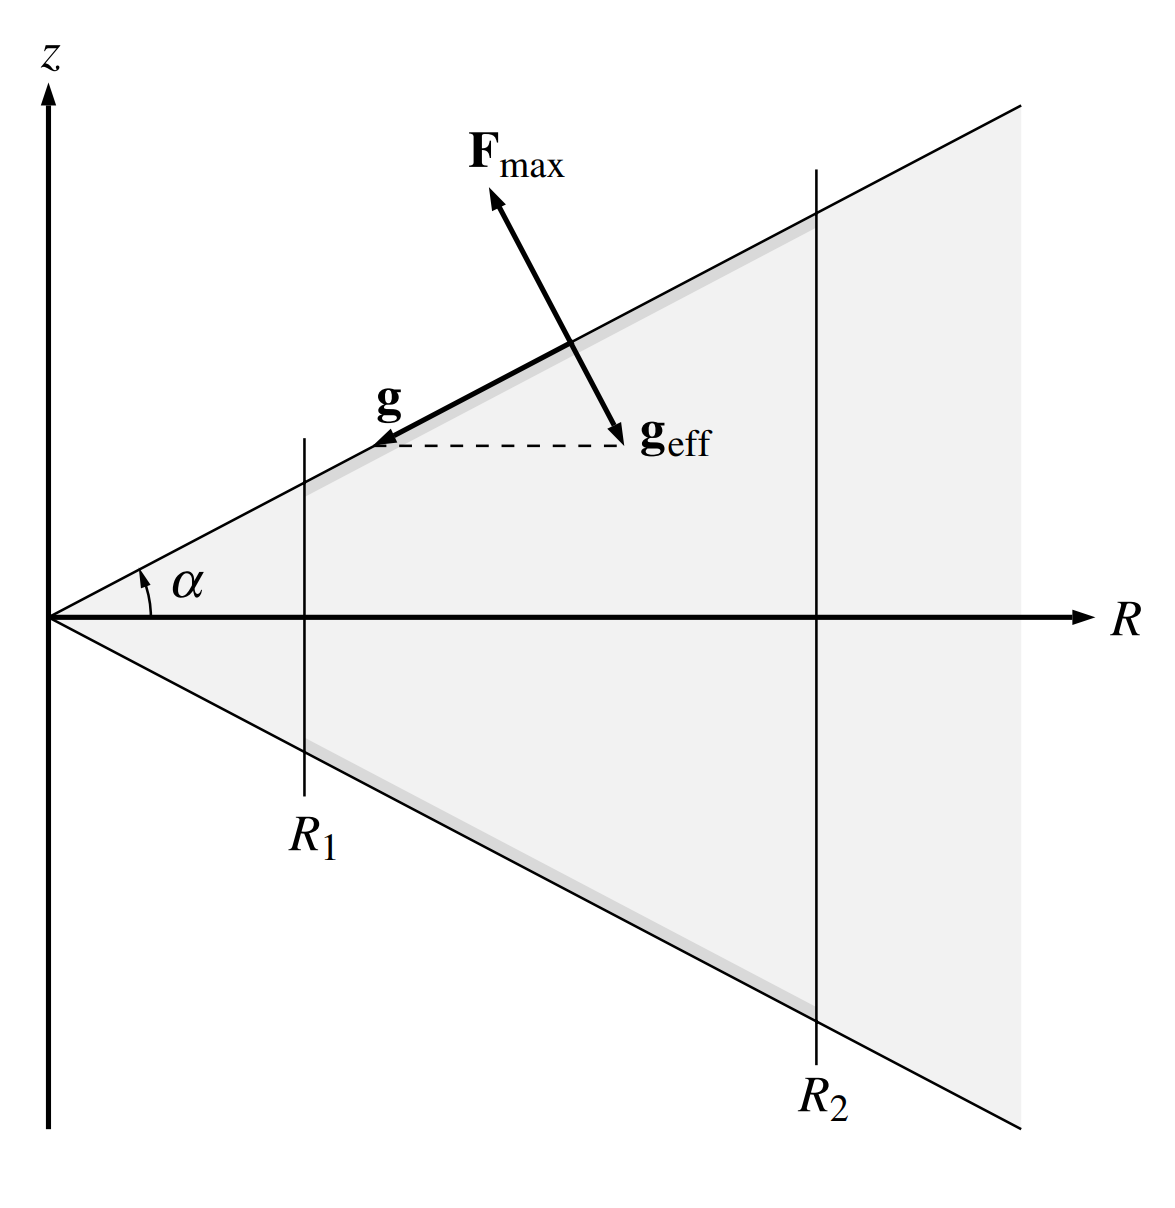
\includegraphics[width=\linewidth]{simple_geometry_geff_Lmax.png}
\caption{Effective surface gravity (rotation and gravity) balance with radiative flux to support the Keplerian rotating thick disk as in \ref{fig:thick-disk-tori-struct} }\label{fig:simple_geometry_geff_Lmax}
\end{figure}
From \ref{eq:L_max_exceed_L_eddingtion_R1R2} it is clear that $L_{max}$ can significantly exceed $L_{Edd}$ if $R_2/R_1$ is large. 

In this appendix we introduced a simple unrealistic thick disk. Although it unrealistic it does include main physical phenomena relevant to realistic thick disk as we assume appears in nature (i.e. AGNs, star formation and stellar merger).
In this research proposal we use computer simulation to produce more realistic thick disk and examine if they can produce some of the main observation features.

\hrulefill

\newpage
\bibliographystyle{abbrvnat}
\bibliography{db}

\end{document}
